\documentclass[25pt, a0paper, landscape, blockverticalspace=5mm]{tikzposter}
\usepackage{cite}
\usepackage{tikz}
\usepackage{graphicx}
\usepackage{caption}
\usepackage{tabularx}
\usepackage{booktabs}
\usepackage{caption}
\usepackage{pgfplots}
\usepackage{url}

\pgfplotsset{compat=1.18}

\usetikzlibrary{arrows.meta, positioning, calc, fit, backgrounds}
\tikzposterlatexaffectionproofoff

\definecolor{managerbg}{RGB}{245,248,252}
\definecolor{managerborder}{RGB}{70,90,120}
\definecolor{semanticcol}{RGB}{255,220,180}
\definecolor{semanticborder}{RGB}{200,120,40}
\definecolor{episodiccol}{RGB}{200,230,255}
\definecolor{episodicborder}{RGB}{40,110,180}
\definecolor{declarativecol}{RGB}{210,240,210}
\definecolor{declarativeborder}{RGB}{40,130,60}
\definecolor{ercol}{RGB}{255,210,210}
\definecolor{erborder}{RGB}{180,50,50}
\definecolor{inputcol}{RGB}{250,240,200}
\definecolor{inputborder}{RGB}{160,130,40}
\definecolor{actioncol}{RGB}{230,210,255}
\definecolor{actionborder}{RGB}{110,60,170}
\definecolor{stevensred}{RGB}{163,38,56}

\usetheme{Autumn}
\colorlet{backgroundcolor}{white}
\colorlet{titlebgcolor}{white}
\colorlet{titlefgcolor}{black}
\colorlet{blocktitlefgcolor}{stevensred}

\makeatletter
\renewenvironment{thebibliography}[1]{%
  \textbf{References:} 
  \let\par\relax\let\newblock\relax % Kills all newlines
  \newcounter{bibcnt}%
  \def\bibitem##1{%
    \stepcounter{bibcnt}%
    \ifnum\value{bibcnt}>1 \quad $\cdot$ \quad \fi % Smaller dot, only prints between items
    [\arabic{bibcnt}] % Prints the number
    \if@filesw\immediate\write\@auxout{\string\bibcite{##1}{\arabic{bibcnt}}}\fi % Keeps \cite{} working
    \ignorespaces
  }%
}{}
\settitle{
    \centering
    % --- LEFT COLUMN: Logos ---
    \begin{minipage}[c]{0.18\linewidth}
        \centering
        \includegraphics[width=0.28\linewidth]{stevens_logo.png}
        \quad
        \includegraphics[width=0.28\linewidth]{icns_logo.png}
    \end{minipage}
    \hfill
    % --- CENTER COLUMN: Title, Authors, Institute ---
    \begin{minipage}[c]{0.6\linewidth}
        \centering
        \color{titlefgcolor}
        {\bfseries \Huge \@title \par}
        \vspace*{1em}
        {\Large \@author \par}
        \vspace*{0.5em}
        {\large \@institute \par}
    \end{minipage}
    \hfill
    % --- RIGHT COLUMN: QR Code ---
    \begin{minipage}[c]{0.18\linewidth}
        \centering
        \hspace*{6em}
        \includegraphics[width=0.3\linewidth]{qrcode.png} \\
        \vspace{0.5em}
        \hspace*{6em}
        \normalsize Scan the QR code to access \\
        \hspace*{6em}
        the full paper and source code.
    \end{minipage}

    \vspace*{1em}
    \noindent\color{black}\rule{\linewidth}{1pt}
    \vspace*{-4cm}
}
\makeatletter

% --- Shrink block body font (titles unaffected) and tighten title-to-body gap ---
\let\TPoldblock\block
\renewcommand{\block}[2]{\TPoldblock{#1}{\vspace{-0.7em}\small #2}}

\title{Tri-Mem: Entropy-Routed Modality Matching for Long-Horizon Agent Memory}
\author{Aniruddha Pandey$^*$, Xuan Li$^*$, Amy Thomas$^*$, Dr. Yue Ning$^\dagger$, Dr. Zining Zhu$^\dagger$}
\institute{Department of Computer Science $\cdot$  Charles V. Schaefer, Jr. School of Engineering and Science $\cdot$ Stevens Institute of Technology}

\begin{document}

\maketitle

\begin{columns}
    % ==================== Left Column ====================
    \column{0.33}
    \block{Motivation: The Homogeneous Context Bottleneck}{
        Current LLM agents force all cognitive functions (rules, history, strict variables) into a single text prompt. This causes cascading failures:
        \begin{itemize}
            \item \textbf{Context Rot:} Critical instructions are lost in the middle of long prompts.~\cite{liu2023lost}
            \item \textbf{Compute Tax:} Forcing the model to re-attend to static rulebooks at every turn.
            \item \textbf{Modality Mismatch:} Verbose text is highly inefficient for spatial or episodic recall.~\cite{deepseekocr,vist2025}
        \end{itemize}

        \vspace{1em}
        \centering
        \resizebox{0.9\linewidth}{!}{% 
            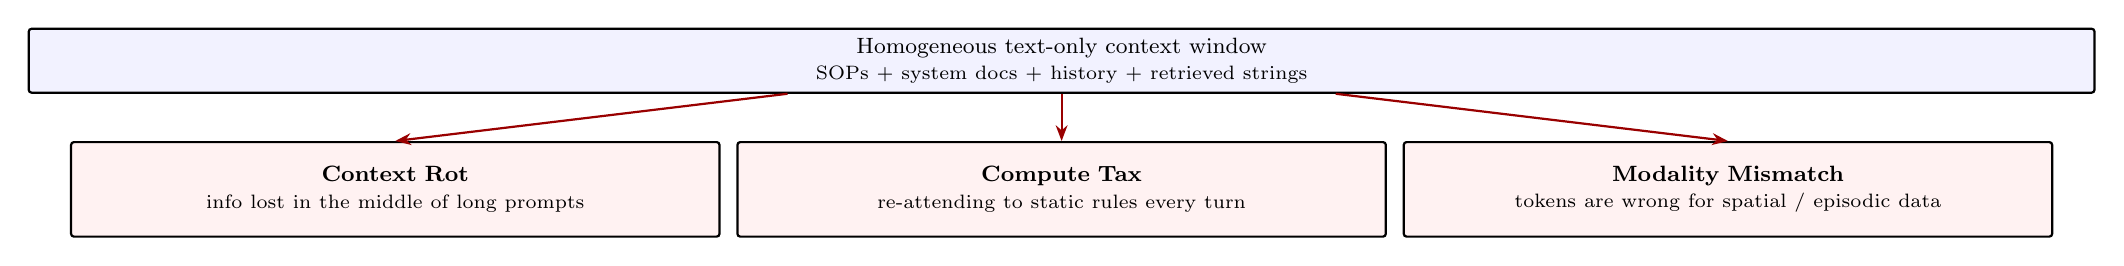
\begin{tikzpicture}[
                font=\footnotesize,
                >={Stealth[length=2mm]},
                node distance=6mm and 2mm,
                ctx/.style={
                        draw, rounded corners=1pt, thick,
                        % FIX 2: Use absolute units inside the diagram
                        text width=26cm,
                        minimum height=7mm,
                        align=center, fill=blue!5
                    },
                failure/.style={
                        draw, rounded corners=1pt, thick,
                        % FIX 2: Use absolute units inside the diagram
                        text width=8cm,
                        minimum height=12mm,
                        align=center, fill=red!5
                    },
                arr/.style={->, thick, red!60!black},
                ]

                \node[ctx] (ctx) {Homogeneous text-only context window\\\scriptsize SOPs $+$ system docs $+$ history $+$ retrieved strings};

                \node[failure, below=of ctx] (tax) {\textbf{Compute Tax}\\\scriptsize re-attending to static rules every turn};
                \node[failure, left=of tax] (rot) {\textbf{Context Rot}\\\scriptsize info lost in the middle of long prompts};
                \node[failure, right=of tax] (mod) {\textbf{Modality Mismatch}\\\scriptsize tokens are wrong for spatial / episodic data};

                \draw[arr] (ctx) -- (rot.north);
                \draw[arr] (ctx) -- (tax.north);
                \draw[arr] (ctx) -- (mod.north);
            \end{tikzpicture}%
        }
        \begin{center}
            \vspace{1em}
            \captionof{figure}{Three cascading failures induced by a homogeneous text-only context window. Tri-Mem binds each function to a different memory modality: rules to MSA, history to the Visual Bus, and exact strings to RAG.}
            \label{fig:motivation}
        \end{center}
    }

    \block{Human Cognitive Inspiration: Tulving's Taxonomy}{
        Tri-Mem is inspired by Tulving's distinction between \emph{episodic} and \emph{semantic} memory~\cite{tulving1972}, augmented with a separate verbatim-fact store for exact alphanumeric strings. Each cognitive function is treated as a distinct system that deserves its own data modality --- not a shared text buffer.

        \vspace{0.4em}
        \footnotesize
        \begin{tabularx}{\linewidth}{@{} l >{\raggedright\arraybackslash}X >{\raggedright\arraybackslash}X @{}}
            \toprule
            \textbf{Human Memory}     & \textbf{Cognitive Role}                  & \textbf{Tri-Mem Layer}     \\
            \midrule
            Semantic                  & Stable knowledge, rules, schemas         & MSA (latent KV chunks)     \\
            Episodic                  & Chronological history, spatial context   & Visual Bus (image patches) \\
            Declarative (verbatim)    & Explicit fact retrieval (exact strings)  & RAG (vector DB tokens)     \\
            \bottomrule
        \end{tabularx}

        \vspace{0.5em}
        \normalsize
        \textbf{Why a 1:1 mapping?} A monolithic text context forces all three roles through the same channel, exposing every function to the same context-rot, compute-tax, and modality-mismatch failures. Modality-matching gives each cognitive role the substrate where its information density is highest and its error mode is bounded.
    }
    \block{The Solution: Modality-to-Function Mapping}{
        Agent memory should not be one-size-fits-all. Prior structured-memory work~\cite{synapse2026,lowcode2025} divides agent memory by function but stays text-centric throughout. Tri-Mem extends the idea: each cognitive function is assigned the data modality whose information-density and fidelity profile best matches it.

        {
            \centering
            \captionof{table}{The Modality-to-Function Matrix. Each Tri-Mem layer is assigned the data modality whose information density and fidelity profile best matches its cognitive function.}
            \label{tab:modality-matrix}

            \vspace{0.5em}
            \footnotesize
            % Use \linewidth to stay inside the column boundaries
            \begin{tabularx}{\linewidth}{@{} l l >{\raggedright\arraybackslash}X >{\raggedright\arraybackslash}X @{}}
                \toprule
                \textbf{Layer}    & \textbf{Modality} & \textbf{Human Analog} & \textbf{Best For}                      \\
                \midrule
                Semantic (MSA)    & Latent KV chunks  & Knowledge / rules     & SOPs, docs, system prompts             \\
                Episodic (V-Bus)  & Visual patches    & Short-term recall     & Chronological history, spatial context \\
                Declarative (RAG) & Discrete tokens   & Fact retrieval        & API keys, IDs, exact strings           \\
                \bottomrule
            \end{tabularx}
        }

        \vspace{1em}
        \textbf{Bridging the Syntactic Action Gap.} Visual compression preserves chronology but blurs exact alphanumeric strings (API keys, object IDs). RAG closes the gap: the Visual Bus flags \emph{what} entity to look up, and the vector store returns the \emph{exact string} losslessly. In AuditBench this fusion drops token cost $58{,}155 \to 7{,}119$ and zeroes both syntactic failures and spatial hallucinations (Table~\ref{tab:metrics}, P3$\to$P4).

        \vspace{0.4em}
        \textbf{Resource ceiling vs.\ architectural ceiling.} The AuditBench cap of \texttt{MAX\_VISUAL\_TILES}$=4$ was a single-GPU OCR-OOM ceiling, not a design limit. Splitting OCR onto a second H100 lifted the cap $4\times$ for the LongMemEval campaign --- the Visual Bus is the modality-correct layer, the GPU was just the bottleneck.
    }

    % ====================  Middle Column ====================
    \column{0.33}
    \block{The Tri-Mem Architecture}{
        Tri-Mem mimics human cognitive structures by splitting memory into three distinct systems:
        \begin{enumerate}
            \item \textbf{Semantic Memory (MSA):} The Rulebook. Static rules and SOPs stored as latent KV chunks.~\cite{evermind2026} Uses document-wise RoPE~\cite{rope2021} to eliminate the per-turn rulebook compute tax.
            \item \textbf{Episodic Working Memory (Visual Bus):} The Scratchpad. Interaction history rendered into highly compressed visual image patches via Segment Optical Caching.~\cite{agentocr2026} Protects chronology and limits context rot.
            \item \textbf{Declarative Memory (RAG):} The Fact Injector. Discrete text tokens via vector DB~\cite{chromadb} to guarantee lossless recall of exact alphanumeric strings.
        \end{enumerate}

        \vspace{1em}
        \begin{center}
            % FIX 1: Explicitly declare the background layer to prevent tikzposter from crashing
            \pgfdeclarelayer{background}
            \pgfsetlayers{background,main}

            \resizebox{0.95\linewidth}{!}{%
                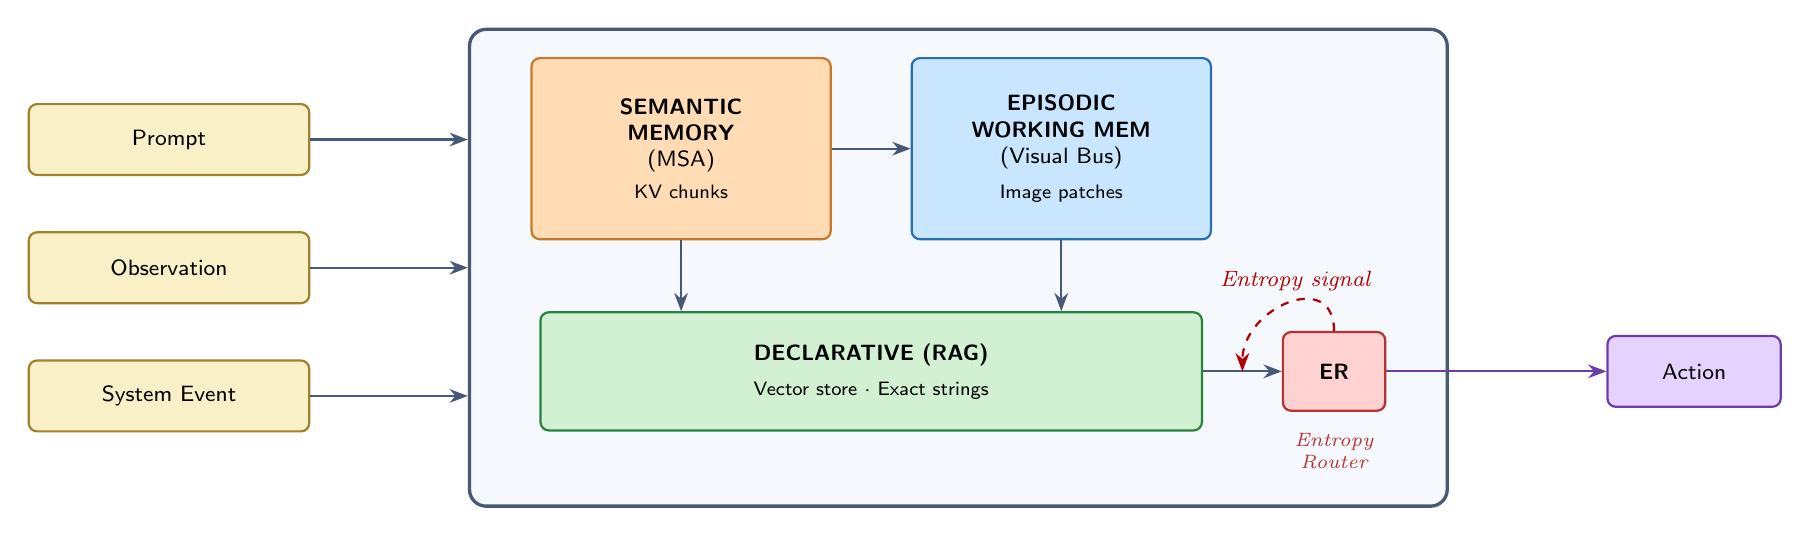
\begin{tikzpicture}[
                        font=\footnotesize\sffamily,
                        >=Stealth,
                        box/.style={
                                rectangle, rounded corners=3pt,
                                draw, thick,
                                align=center,
                                inner sep=8pt
                            },
                        input/.style={
                                box, fill=inputcol, draw=inputborder,
                                text width=3cm, minimum height=0.9cm
                            },
                        memblock/.style={box, minimum width=3.8cm, minimum height=2.3cm, inner sep=10pt},
                        smallbox/.style={
                                box, minimum width=1.3cm, minimum height=1cm,
                                fill=ercol, draw=erborder
                            },
                        action/.style={
                                box, fill=actioncol, draw=actionborder,
                                minimum width=2.2cm, minimum height=0.9cm
                            },
                        arrow/.style={->, thick, draw=managerborder},
                        dataflow/.style={->, thick, draw=red!70!black, dashed}
                    ]

                    % ===== Semantic & Episodic Memories (Top Row) =====
                    \node[memblock, fill=semanticcol, draw=semanticborder] (semantic) {
                    \textbf{SEMANTIC}\\\textbf{MEMORY}\\(MSA)\\[2pt]
                    {\scriptsize KV chunks}
                    };

                    \node[memblock, fill=episodiccol, draw=episodicborder, right=1cm of semantic] (episodic) {
                    \textbf{EPISODIC}\\\textbf{WORKING MEM}\\(Visual Bus)\\[3pt]
                    {\scriptsize Image patches}
                    };

                    % ===== Declarative Memory (Bottom Row) =====
                    \path (semantic.south east) -- (episodic.south west) coordinate[midway] (gap);
                    \node[memblock, fill=declarativecol, draw=declarativeborder,
                    anchor=north, minimum width=8.4cm, minimum height=1.5cm,
                    below=0.9cm of gap] (declarative) {
                    \textbf{DECLARATIVE (RAG)}\\[3pt]
                    {\scriptsize Vector store $\cdot$ Exact strings}
                    };

                    % ===== ER Node =====
                    \node[smallbox, right=1cm of declarative] (er) {\textbf{ER}};
                    \node[below=0.15cm of er, font=\scriptsize\itshape, align=center, text=erborder] (erlabel) {Entropy\\Router};

                    % ===== Manager Background =====
                    \begin{scope}[on background layer]
                        \node[
                            draw=managerborder, very thick, rounded corners=6pt,
                            fill=managerbg,
                            fit=(semantic)(episodic)(declarative)(er)(erlabel),
                            inner xsep=22pt, inner ysep=10pt
                        ] (manager) {};
                    \end{scope}

                    % ===== Input Nodes (all same width via text width) =====
                    \node[input, left=2cm of manager.west] (obs) {Observation };
                    \node[input, above=0.7cm of obs] (prompt) {Prompt};
                    \node[input, below=0.7cm of obs] (sysev) {System Event};

                    % ===== Action Node =====
                    \node[action, right=2cm of manager.east |- er] (action) {Action};

                    % ===== Arrows =====
                    % Inputs to Manager
                    \draw[arrow] (prompt.east) -- (manager.west |- prompt.east);
                    \draw[arrow] (obs.east) -- (manager.west |- obs.east);
                    \draw[arrow] (sysev.east) -- (manager.west |- sysev.east);

                    % Internal connections
                    \draw[arrow] (semantic.east) -- (episodic.west);
                    \draw[arrow] (semantic.south) -- (semantic.south |- declarative.north);
                    \draw[arrow] (episodic.south) -- (episodic.south |- declarative.north);

                    % Declarative to ER
                    \path (declarative.east) -- (er.west) coordinate[midway] (mid_decl_er);
                    \draw[arrow] (declarative.east) -- (er.west);

                    % ER to Action
                    \draw[arrow, draw=actionborder] (er.east) -- (action.west);

                    % Entropy Feedback - red dashed curve from ER back up to Episodic area
                    % \draw[dataflow] (er.north) .. controls +(up:1.5cm) and +(right:1.2cm) ..
                    %     node[pos=0.45, above, font=\scriptsize\itshape, text=red!70!black] {Entropy signal}
                    %     (episodic.south east);

                    % Entropy Feedback (Curved arrow looping back to the ER input line)
                    \draw[dataflow] (er.north) .. controls +(up:0.8cm) and +(up:0.8cm) ..
                    node[pos=0.45, above, font=\footnotesize\itshape, text=red!70!black] {Entropy signal}
                    (mid_decl_er);

                \end{tikzpicture}
            }
            \vspace{0.5em}
            \captionof{figure}{The Tri-Mem manager. Incoming streams (prompt, observation, system event) flow through three modality-distinct memory layers --- Semantic Memory (MSA, KV chunks), Episodic Working Memory (Visual Bus, image patches), and Declarative Memory (RAG) --- coordinated by the Entropy Router (ER), which uses a single-token probe to decide per turn which layers to consult.}
            \label{fig:architecture}
        \end{center}

    }

    \block{Uncertainty-Guided Entropy Routing}{
        \begin{equation}
            H(X) = -\sum_{x \in \mathcal{X}} p(x) \log_2 p(x).
        \end{equation}
        \vspace{1em}

        Instead of costly LLM "think-aloud" prompting to decide which memory to use, Tri-Mem uses raw logit confidence (Shannon Entropy)~\cite{shannon1948} as a single-token probe (informed by Bayesian belief updating~\cite{googlebayes2026}):

        \vspace{1em}
        \begin{center}
            % --- ENTIRE FIGURE IN ONE MASSIVE HORIZONTAL TIKZPICTURE ---
            \resizebox{\linewidth}{!}{%
                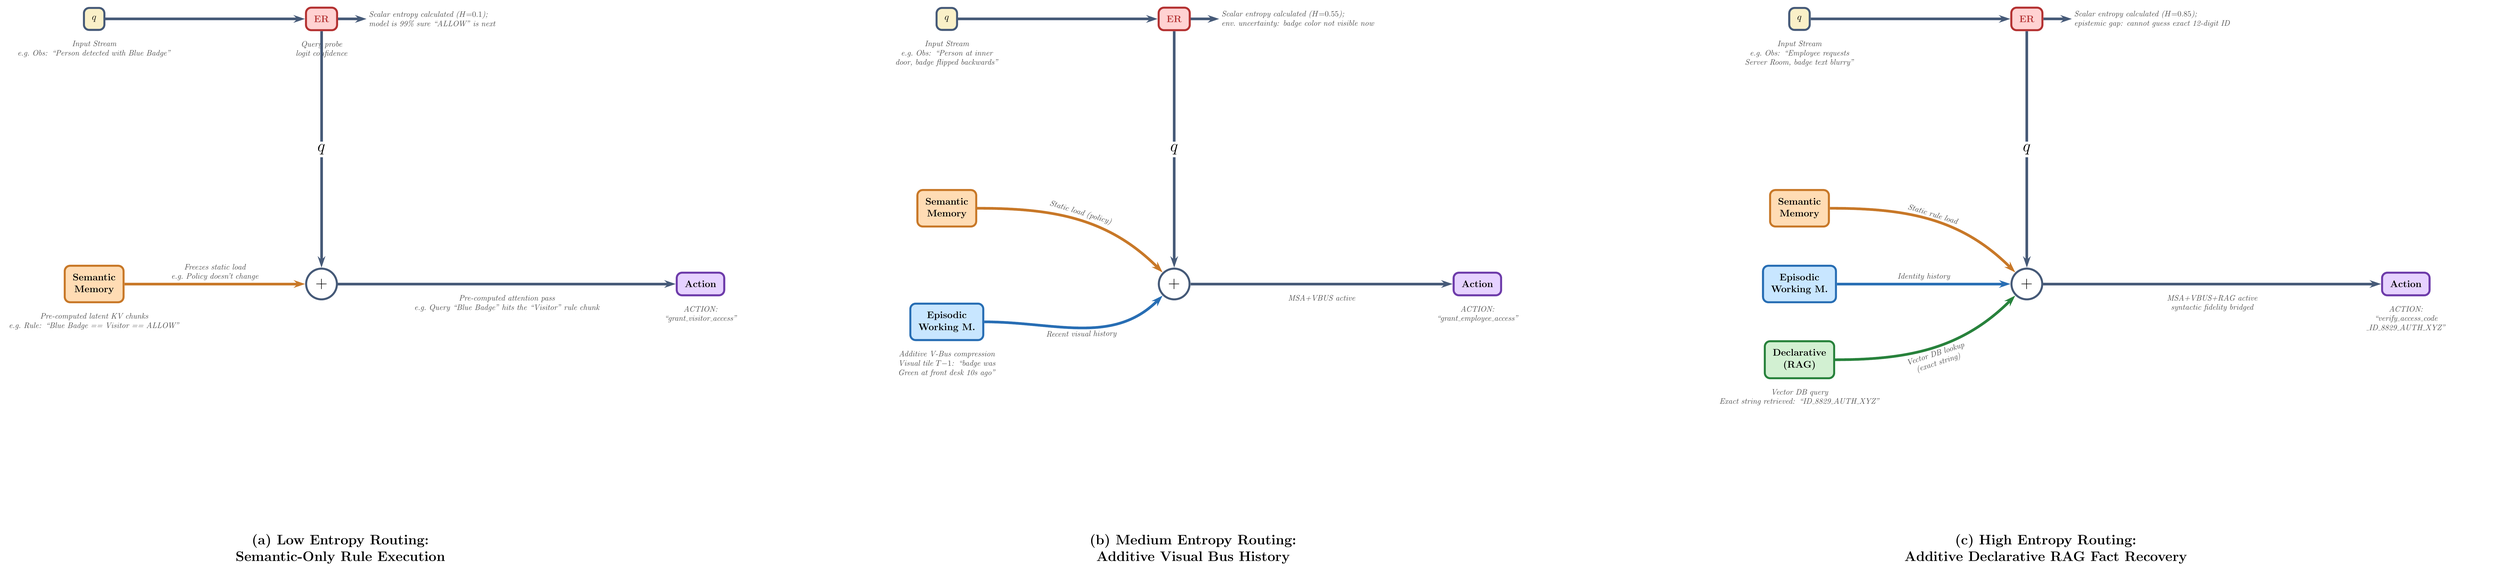
\begin{tikzpicture}[
                    font=\sffamily,
                    >={Stealth[length=6mm, width=4mm]},
                    % KNOB 1: Main Box Fonts (changed \normalsize to \Large)
                    mainnode/.style={rectangle, rounded corners=8pt, draw=managerborder, line width=3pt, inner sep=12pt, align=center, font=\Large\bfseries},
                    % KNOB 2: Sub-label Fonts (changed \footnotesize to \large)
                    sublabel/.style={align=center, font=\large\itshape, text=black!75},
                    arrow/.style={->, line width=4pt, draw=managerborder}
                    ]

                    % ==========================================
                    % (a) LOW ENTROPY (Left)
                    % ==========================================
                    \begin{scope}[shift={(0,0)}]
                        \node[mainnode, fill=inputcol] (q) at (0,0) {$q$};
                        \node[mainnode, fill=ercol, draw=erborder, text=erborder] (er) at (12,0) {ER};
                        \node[sublabel, right=1.5cm of er, text width=12cm, align=left] (entropy) {Scalar entropy calculated ($H{=}0.1$);\\ model is 99\% sure ``ALLOW'' is next};

                        \node[mainnode, fill=semanticcol, draw=semanticborder] (sem) at (0,-14) {Semantic\\Memory};
                        \node[circle, draw=managerborder, line width=3pt, fill=white, inner sep=8pt, font=\Huge\bfseries] (plus) at (12,-14) {$+$};
                        \node[mainnode, fill=actioncol, draw=actionborder] (action) at (32,-14) {Action};

                        % Labels (widened text width to prevent stacking with larger fonts)
                        \node[sublabel, below=0.4cm of q, text width=9cm] {Input Stream\\e.g.\ Obs: ``Person detected with Blue Badge''};
                        \node[sublabel, below=0.4cm of er, text width=8cm] {Query probe\\logit confidence};
                        \node[sublabel, below=0.4cm of sem, text width=9cm] {Pre-computed latent KV chunks\\ e.g.\ Rule: ``Blue Badge == Visitor == ALLOW''};
                        \node[sublabel, below=0.4cm of action, text width=9cm] {ACTION:\\``grant\_visitor\_access''};

                        % Arrows
                        \draw[arrow] (q) -- (er);
                        \draw[arrow] (er) -- (entropy.west |- er);
                        \draw[arrow] (er) -- node[midway, fill=white, font=\Huge\bfseries, inner sep=4pt] {$q$} (plus);
                        \draw[arrow, draw=semanticborder] (sem) -- node[sublabel, above, text width=9cm] {Freezes static load\\e.g.\ Policy doesn't change} (plus);
                        \draw[arrow] (plus) -- node[sublabel, below, yshift=-4mm, text width=12cm] {Pre-computed attention pass\\ e.g.\ Query ``Blue Badge'' hits the ``Visitor'' rule chunk} (action);

                        \node[font=\huge\bfseries, text=black, align=center, text width=26cm] at (13, -28) {(a) Low Entropy Routing:\\Semantic-Only Rule Execution};
                    \end{scope}

                    % ==========================================
                    % (b) MEDIUM ENTROPY (Center)
                    % Shifted by 45 to give massive breathing room between panels
                    % ==========================================
                    \begin{scope}[shift={(45,0)}]
                        \node[mainnode, fill=inputcol] (q) at (0,0) {$q$};
                        \node[mainnode, fill=ercol, draw=erborder, text=erborder] (er) at (12,0) {ER};
                        \node[sublabel, right=1.5cm of er, text width=12cm, align=left] (entropy) {Scalar entropy calculated ($H{=}0.55$);\\ env.\ uncertainty: badge color not visible now};

                        \node[mainnode, fill=semanticcol, draw=semanticborder] (sem) at (0,-10) {Semantic\\Memory};
                        \node[mainnode, fill=episodiccol, draw=episodicborder] (epi) at (0,-16) {Episodic\\Working M.};

                        \node[circle, draw=managerborder, line width=3pt, fill=white, inner sep=8pt, font=\Huge\bfseries] (plus) at (12,-14) {$+$};
                        \node[mainnode, fill=actioncol, draw=actionborder] (action) at (28,-14) {Action};

                        % Labels
                        \node[sublabel, below=0.4cm of q, text width=9cm] {Input Stream\\e.g.\ Obs: ``Person at inner door, badge flipped backwards''};
                        \node[sublabel, below=0.4cm of epi, text width=10cm] {Additive V-Bus compression\\Visual tile $T{-}1$: ``badge was Green at front desk 10s ago''};
                        \node[sublabel, below=0.4cm of action, text width=9cm] {ACTION:\\``grant\_employee\_access''};

                        % Arrows
                        \draw[arrow] (q) -- (er);
                        \draw[arrow] (er) -- (entropy.west |- er);
                        \draw[arrow] (er) -- node[midway, fill=white, font=\Huge\bfseries, inner sep=4pt] {$q$} (plus);

                        \draw[arrow, draw=semanticborder] (sem.east) to[out=0, in=135] node[sublabel, above, sloped, text width=7cm] {Static load (policy)} (plus.135);
                        \draw[arrow, draw=episodicborder] (epi.east) to[out=0, in=225] node[sublabel, below, sloped, text width=8cm] {Recent visual history} (plus.225);

                        \draw[arrow] (plus) -- node[sublabel, below, yshift=-4mm, text width=11cm] {MSA+VBUS active} (action);

                        % TITLE POSITION & FONT
                        \node[font=\huge\bfseries, text=black, align=center, text width=26cm] at (13, -28) {(b) Medium Entropy Routing:\\Additive Visual Bus History};
                    \end{scope}

                    % ==========================================
                    % (c) HIGH ENTROPY (Right)
                    % Shifted by 90
                    % ==========================================
                    \begin{scope}[shift={(90,0)}]
                        \node[mainnode, fill=inputcol] (q) at (0,0) {$q$};
                        \node[mainnode, fill=ercol, draw=erborder, text=erborder] (er) at (12,0) {ER};
                        \node[sublabel, right=1.5cm of er, text width=12cm, align=left] (entropy) {Scalar entropy calculated ($H{=}0.85$);\\ epistemic gap: cannot guess exact 12-digit ID};

                        \node[mainnode, fill=semanticcol, draw=semanticborder] (sem) at (0,-10) {Semantic\\Memory};
                        \node[mainnode, fill=episodiccol, draw=episodicborder] (epi) at (0,-14) {Episodic\\Working M.};
                        \node[mainnode, fill=declarativecol, draw=declarativeborder] (rag) at (0,-18) {Declarative\\(RAG)};

                        \node[circle, draw=managerborder, line width=3pt, fill=white, inner sep=8pt, font=\Huge\bfseries] (plus) at (12,-14) {$+$};
                        \node[mainnode, fill=actioncol, draw=actionborder] (action) at (32,-14) {Action};

                        % Labels
                        \node[sublabel, below=0.4cm of q, text width=9cm] {Input Stream\\e.g.\ Obs: ``Employee requests Server Room, badge text blurry''};
                        \node[sublabel, below=0.4cm of rag, text width=10cm] {Vector DB query\\Exact string retrieved: ``ID\_8829\_AUTH\_XYZ''};
                        \node[sublabel, below=0.4cm of action, text width=9cm] {ACTION:\\``verify\_access\_code\\\_ID\_8829\_AUTH\_XYZ''};

                        % Arrows
                        \draw[arrow] (q) -- (er);
                        \draw[arrow] (er) -- (entropy.west |- er);
                        \draw[arrow] (er) -- node[midway, fill=white, font=\Huge\bfseries, inner sep=4pt] {$q$} (plus);

                        \draw[arrow, draw=semanticborder] (sem.east) to[out=0, in=135] node[sublabel, above, sloped, text width=6cm] {Static rule load} (plus.135);
                        \draw[arrow, draw=episodicborder] (epi.east) -- node[sublabel, above] {Identity history} (plus.west);
                        \draw[arrow, draw=declarativeborder] (rag.east) to[out=0, in=225] node[sublabel, below, sloped, text width=7cm] {Vector DB lookup\\(exact string)} (plus.225);

                        \draw[arrow] (plus) -- node[sublabel, below, yshift=-4mm, text width=12cm] {MSA+VBUS+RAG active\\syntactic fidelity bridged} (action);

                        % TITLE POSITION & FONT
                        \node[font=\huge\bfseries, text=black, align=center, text width=26cm] at (13, -28) {(c) High Entropy Routing:\\Additive Declarative RAG Fact Recovery};
                    \end{scope}
                \end{tikzpicture}%
            }

            \captionof{figure}{Tri-Mem Additive Memory Gating Architecture. The progression above illustrates how the Entropy Router (ER) dynamically gates three functional memory layers based on intrinsic model uncertainty, forming additive memory bands of increasing cognitive load and fidelity.}
            \label{fig:combined-entropy}
        \end{center}

        \vspace{0.4em}
        \textbf{Threshold calibration.} A prior choice of $0.3$ for the LOW boundary never fired in practice --- the minimum observed first-token entropy floored at $\approx 0.33$ on cached SOP transitions (e.g.\ \texttt{access compliance\_dashboard} after a fresh download). Raising the boundary to $0.4$ yields a true ternary partition: $\approx 5/60/35\%$ MSA-only / MSA$+$VBus / MSA$+$VBus$+$RAG across the seven-task suite. The LOW band reliably fires on truly cached transitions where the next system in the SOP is already in the model's working state; thresholds are regression-tested against pinned probe entropies in the unit-test suite.
    }

    % ====================  Right Column ====================
    \column{0.34}
    \block{Experimental Validations}{
        \textbf{NovaCorp AuditBench: Solving The Token Paradox}
        \vspace{0.5cm}\\
        Stress-testing semantic rule-following and episodic recall on a long-horizon SaaS auditing task.

            {
                \centering
                \captionof{table}{Performance Metrics on NovaCorp AuditBench (Single Task: Vendor Invoice Audit)}
                \label{tab:metrics}

                \vspace{0.5em}
                \footnotesize
                % Use \linewidth to stay inside the column boundaries
                \begin{tabularx}{\linewidth}{@{} l X r r r r r r @{}}
                    \toprule
                    \textbf{Metric}                   & \textbf{What It Measures}                        & \textbf{Phase 1} & \textbf{Phase 2} & \textbf{Phase 3} & \textbf{Phase 4} & \textbf{Phase 5} & \textbf{Phase 6}       \\
                                                      &                                                  & (Baseline)       & (RAG)            & (Visual Bus)     & (VBus+RAG)       & (MSA)            & (Tri-Mem)              \\
                    \midrule
                    \textbf{Success Rate}             & Task completion percentage                       & 1.0              & 1.0              & 1.0              & 1.0              & 1.0              & 1.0                    \\
                    \textbf{Total Token Cost}         & Total tokens (in + out) over task                & 45,169           & 262,147          & 58,155           & 7,119            & 29,026           & 31,606                 \\
                    \textbf{Resolution Length}        & Total turns to solve (lower is better)           & 41               & 48               & 36               & 7                & 6                & 6                      \\
                    \textbf{Syntactic Failure}        & Environment ``Syntax error'' responses           & 0                & 0                & 6                & 0                & 0                & 0                      \\
                    \textbf{Spatial Hallucination}    & Interacting with non-reachable systems           & 25               & 34               & 19               & 0                & 0                & 0                      \\
                    \textbf{Memory Source}            & Modality routed per turn                         & text             & rag              & vbus             & vb+rag           & msa              & 17/67/17\%$^{\dagger}$ \\
                    \textbf{Avg Latency per Turn (s)} & Inference + (probe + OCR + RAG)                  & ---              & ---              & 2.7              & 1.7              & 1.2              & 0.9$^{\ddagger}$       \\
                    \textbf{Wall-Clock Duration (s)}  & Time from \texttt{reset()} to \texttt{done=True} & ---              & ---              & 817.5            & 93.5             & 19.5             & 38.1                   \\
                    \bottomrule
                    \multicolumn{8}{@{}l}{\footnotesize $^{\dagger}$ msa / msa+vbus / msa+vbus+rag band split for Tri-Mem on this single task; the seven-task aggregate is 5\,/\,60\,/\,35\%.}                                   \\
                    \multicolumn{8}{@{}l}{\footnotesize $^{\ddagger}$ MED-band steady-state average; LOW-band turns drop to $\approx 0.5$\,s because the Visual Bus OCR pass is skipped. Cold-start turn 0 is excluded.}
                \end{tabularx}
            }

        \begin{center}
            \begin{minipage}[c]{0.58\linewidth}
                \centering
                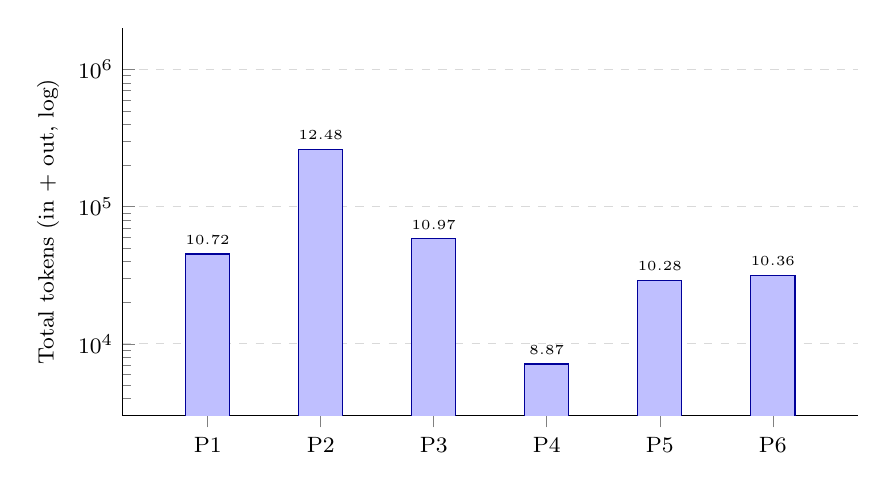
\begin{tikzpicture}
                    \begin{axis}[
                            width=0.9\linewidth, height=6.5cm, % Reduced width slightly to cluster bars
                            ybar, bar width=16pt, % Increased bar width to close the gaps
                            enlarge x limits=0.15,
                            ymode=log, ymin=3000, ymax=2000000,
                            ylabel={Total tokens (in $+$ out, log)},
                            symbolic x coords={P1, P2, P3, P4, P5, P6},
                            xtick=data,
                            axis x line*=bottom, % Removes top bounding line
                            axis y line*=left,   % Removes right bounding line
                            xticklabel style={font=\footnotesize},
                            yticklabel style={font=\footnotesize},
                            ylabel style={font=\footnotesize},
                            nodes near coords,
                            nodes near coords style={font=\tiny, anchor=south}, % Horizontal, anchored to sit on top of the bar
                            every node near coord/.append style={
                                    /pgf/number format/.cd, fixed, 1000 sep={,}
                                },
                            ymajorgrids, major grid style={dashed, gray!30}, % Softened, dashed grid lines
                        ]
                        \addplot[fill=blue!25, draw=blue!60!black]
                        coordinates {
                                (P1, 45169) (P2, 262147) (P3, 58155)
                                (P4, 7119) (P5, 29026) (P6, 31606)
                            };
                    \end{axis}
                \end{tikzpicture}
                \vspace{0.5em}
                \captionof{figure}{Total token cost per AuditBench task by phase (log scale). \textbf{P1}: text-only baseline. \textbf{P2}: continuous RAG inflates context to 262\,k. \textbf{P3}: Visual Bus alone collapses tokens but introduces six syntactic failures (Table~\ref{tab:metrics}). \textbf{P4}: Visual Bus $+$ RAG hits the floor at 7\,k tokens by gating exact-string lookups behind the visual layer's entity flags. \textbf{P5}: MSA prefix-cache. \textbf{P6}: full Tri-Mem with the entropy router pays $\approx 9\%$ over P5 in exchange for adaptive per-turn layer selection.}
                \label{fig:auditbench-tokens}
            \end{minipage}\hfill
            \begin{minipage}[c]{0.38\linewidth}
                \centering
                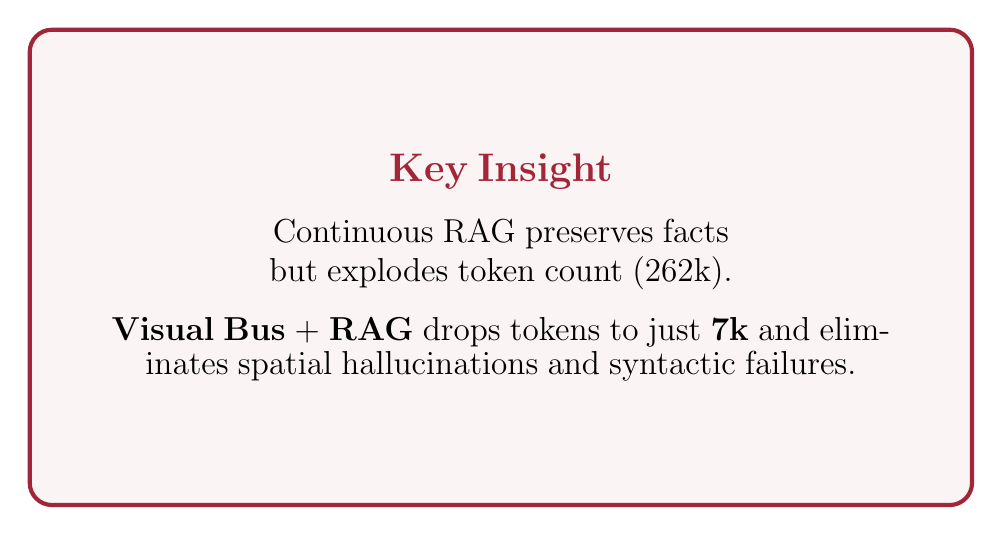
\begin{tikzpicture}
                    \node[
                        draw=stevensred,
                        fill=stevensred!5,
                        line width=1.5pt,
                        rounded corners=8pt,
                        inner xsep=15pt,
                        inner ysep=45pt,
                        text width=0.9\linewidth,
                        align=center
                    ] {
                        {\Large\textbf{\color{stevensred} Key Insight}}\\[0.8em]
                        \large Continuous RAG preserves facts but explodes token count (262k).\\[0.8em]
                        \textbf{Visual Bus $+$ RAG} drops tokens to just \textbf{7k} and eliminates spatial hallucinations and syntactic failures.
                    };
                \end{tikzpicture}
            \end{minipage}
        \end{center}

        \textbf{Validation on LongMemEval~\cite{longmemeval2024,longmemevalrepo}}
        \vspace{0.5cm}\\
        Evaluating on a public benchmark for conversational long-term memory (single-shot Q\&A).

        \begin{center}
            \begin{minipage}[t]{0.48\linewidth}
                \centering
                \captionof{table}{Tri-Mem on LongMemEval Oracle Split (Dispatch-Aware Judge, $n=500$)}
                \label{tab:longmem-oracle}
                \vspace{0.5em}
                \footnotesize
                \begin{tabular}{@{}lrr@{}}
                    \toprule
                    \textbf{Question Category}    & \textbf{n} & \textbf{Accuracy}                                 \\
                    \midrule
                    single-session-assistant      & 56         & \textbf{100.0\%}                                  \\
                    single-session-user           & 70         & 88.6\%                                            \\
                    knowledge-update              & 78         & 83.3\%                                            \\
                    temporal-reasoning            & 133        & 81.2\%                                            \\
                    multi-session                 & 133        & 75.2\%                                            \\
                    single-session-preference     & 30         & 53.3\%$^{\dagger}$                                \\
                    \midrule
                    Factual subset (5 categories) & 470        & 83.2\%                                            \\
                    \textbf{Overall (all 6)}      & 500        & \textbf{81.4\%}                                   \\
                    \bottomrule
                    \multicolumn{3}{@{}l}{\footnotesize $^{\dagger}$ Rubric-judge score; the strict factual judge} \\
                    \multicolumn{3}{@{}l}{\footnotesize \quad scored this category at 6.7\% (see \S VI-E).}
                \end{tabular}
            \end{minipage}\hfill
            \begin{minipage}[t]{0.48\linewidth}
                \centering
                \captionof{table}{Tri-Mem on LongMemEval s\_cleaned (Dispatch-Aware Judge, $n=500$). Observed rows are scored on completed questions; projected rows apply the per-category retrieval delta measured on the completed slice plus the oracle reference.}
                \label{tab:longmem-s}
                \vspace{0.5em}
                \footnotesize
                \begin{tabular}{@{}lrrl@{}}
                    \toprule
                    \textbf{Question Category}    & \textbf{n} & \textbf{Accuracy}           & \textbf{Status}       \\
                    \midrule
                    single-session-user           & 70         & 81.4\%                      & observed (full)       \\
                    multi-session                 & 133        & 68.4\%                      & observed ($n$=19/133) \\
                    single-session-assistant      & 56         & ${\sim}\,$95\%              & projected             \\
                    knowledge-update              & 78         & ${\sim}\,$77\%              & projected             \\
                    temporal-reasoning            & 133        & ${\sim}\,$74\%              & projected             \\
                    single-session-preference     & 30         & ${\sim}\,$53\%              & projected             \\
                    \midrule
                    Factual subset (5 categories) & 470        & ${\sim}\,$78\%              & blended               \\
                    \textbf{Overall (all 6)}      & 500        & \textbf{${\sim}\,$75--76\%} & blended               \\
                    \bottomrule
                \end{tabular}
            \end{minipage}
        \end{center}

        \vspace{0.4em}
        \textbf{Where Tri-Mem struggles: multi-session friction.} Multi-session at 75.2\% is the lowest factual category. Failure inspection finds two recurring patterns: (a) the relevant fact lives in a session that did not make the MSA top-$k{=}4$ selection --- either an embedding-similarity miss or genuine top-$k$ insufficiency; and (b) the model produces partial recall but contradicts itself across reasoning steps, suggesting verbose CoT is in tension with the precision required for cross-session synthesis. The post-hoc extraction pass (\S VI-D of the paper) recovers some of (b); top-$k$ tuning is left to future work.
    }

\end{columns}

% Pull the next block up to tighten the gap after the columns.
\makeatletter
\addtolength{\TP@blocktop}{1cm} % POSITIVE values move the block UP; tune as needed
\makeatother

\block{Implementation Findings \& Future Work}{
    \textbf{Three lessons from the LongMemEval campaign that generalize to any modality-routed agent.}
    \vspace{0.4em}

    \noindent
    \begin{minipage}[t]{0.32\linewidth}
        \textbf{1. GPU-resource isolation matters.} Co-locating vLLM~\cite{vllm2023} (answer LLM, Qwen3.6-35B-A3B~\cite{qwen3report}) and GLM-OCR~\cite{glmocr2026} on a single H100 NVL via Hugging Face Accelerate~\cite{accelerate} forced \texttt{MAX\_VISUAL\_TILES}$=4$ to avoid OCR OOM. Pinning OCR to \texttt{cuda:1} for LongMemEval lifted the cap $4\times$ to $16$ --- a resource ceiling, not an architectural one.
    \end{minipage}\hfill
    \begin{minipage}[t]{0.32\linewidth}
        \textbf{2. Thinking-mode is per call site, not global.} Qwen3.x's \texttt{<think>} preface helps the answer pass (date arithmetic, multi-session synthesis) but \emph{harms} the entropy probe (collapses the first-token band signal) and the LLM judge (yes/no verdict). Tri-Mem applies it independently: \textbf{probe OFF, answer ON, judge OFF}.
    \end{minipage}\hfill
    \begin{minipage}[t]{0.32\linewidth}
        \textbf{3. Per-category judge dispatch.} A strict paraphrase-tolerant judge scored \texttt{single-session-preference} at 6.7\%; switching to a rubric judge \emph{for that category alone} lifted it to 53.3\% --- an order-of-magnitude correction that was a \emph{judge artifact}, not an architectural failure.
    \end{minipage}

    \vspace{0.6em}
    \textbf{Future work.} (i) Bayesian recalibration of the entropy thresholds against per-category probe distributions on LongMemEval rather than only AuditBench. (ii) A preference-tuned answer prompt to close the residual rubric-judge gap. (iii) Extension to multi-agent settings in which the Visual Bus serves as a shared episodic medium across cooperating agents.
}

\makeatletter
\addtolength{\TP@blocktop}{0.5cm} % POSITIVE values move the block UP
\makeatother

% ==================== Global Footer ====================
\block{}{
    \tiny % Makes the text small and unobtrusive

    $^*$Student Researcher \quad $^\dagger$Faculty Advisor

    % --- The Bibliography ---
    \begin{thebibliography}{9}

        \bibitem{synapse2026}
        A. G. Yadav, V. Dherange, and K. Shivam, ``Project Synapse: A Hierarchical Multi-Agent Framework with Hybrid Memory for Autonomous Resolution of Last-Mile Delivery Disruptions,'' \textit{arXiv preprint arXiv:2601.08156}, 2026.

        \bibitem{lowcode2025}
        J. Xu, ``Memory Management and Contextual Consistency for Long-Running Low-Code Agents,'' \textit{arXiv preprint arXiv:2509.25250}, 2025.

        \bibitem{deepseekocr}
        H. Wei, Y. Sun, and Y. Li, ``DeepSeek-OCR: Contexts Optical Compression,'' \textit{arXiv preprint arXiv:2510.18234}, 2025.

        \bibitem{agentocr2026}
        L. Feng, F. Yang, F. Chen, X. Cheng, H. Xu, Z. Wan, M. Yan, and B. An, ``AgentOCR: Reimagining Agent History via Optical Self-Compression,'' \textit{arXiv preprint arXiv:2601.04786}, 2026.

        \bibitem{vist2025}
        L. Xing, A. J. Wang, R. Yan, X. Shu, and J. Tang, ``Vision-centric Token Compression in Large Language Model,'' \textit{arXiv preprint arXiv:2502.00791}, 2025.

        \bibitem{evermind2026}
        Y. Chen, R. Chen, S. Yi, X. Zhao, X. Li, J. Zhang, J. Sun, C. Hu, Y. Han, L. Bing, Y. Deng, and T. Chen, ``MSA: Memory Sparse Attention for Efficient End-to-End Memory Model Scaling to 100M Tokens,'' \textit{arXiv preprint arXiv:2603.23516}, 2026.

        \bibitem{googlebayes2026}
        S. van Steenkiste and T. Linzen, ``Teaching LLMs to reason like Bayesians,'' Google Research Blog, Mar. 4, 2026.

        \bibitem{liu2023lost}
        N. F. Liu, K. Lin, J. Hewitt, A. Paranjape, M. Bevilacqua, S. Petroni, and P. Liang, ``Lost in the middle: How language models use long contexts,'' \textit{arXiv preprint arXiv:2307.03172}, 2023.

        \bibitem{longmemeval2024}
        D. Wu, H. Wang, W. Yu, Y. Zhang, K.-W. Chang, and D. Yu, ``LongMemEval: Benchmarking Chat Assistants on Long-Term Interactive Memory,'' \textit{arXiv preprint arXiv:2410.10813}, 2024.

        \bibitem{longmemevalrepo}
        D. Wu \textit{et al.}, ``LongMemEval'' (software and dataset). \url{https://github.com/xiaowu0162/LongMemEval}, accessed 2026-05.

        \bibitem{vllm2023}
        W. Kwon, Z. Li, S. Zhuang, Y. Sheng, L. Zheng, C. H. Yu, J. E. Gonzalez, H. Zhang, and I. Stoica, ``Efficient Memory Management for Large Language Model Serving with PagedAttention,'' in \textit{Proc. 29th Symp.\ on Operating Systems Principles (SOSP)}, 2023. arXiv:2309.06180.

        \bibitem{rope2021}
        J. Su, Y. Lu, S. Pan, A. Murtadha, B. Wen, and Y. Liu, ``RoFormer: Enhanced Transformer with Rotary Position Embedding,'' \textit{arXiv preprint arXiv:2104.09864}, 2021.

        \bibitem{qwen3report}
        Qwen Team, ``Qwen3 Technical Report,'' \textit{arXiv preprint arXiv:2505.09388}, Alibaba Cloud, 2025.

        \bibitem{glmocr2026}
        Z.ai (Zhipu AI) GLM-OCR Team, ``GLM-OCR Technical Report,'' \textit{arXiv preprint arXiv:2603.10910}, 2026.

        \bibitem{chromadb}
        Chroma, ``Chroma: the AI-native open-source embedding database.'' \url{https://www.trychroma.com/}, accessed 2026-05.

        \bibitem{accelerate}
        S. Gugger, L. Debut, T. Wolf, P. Schmid, Z. Mueller, S. Mangrulkar, M. Sun, and B. Bossan, ``Accelerate: Training and inference at scale made simple, efficient and adaptable,'' Hugging Face, \url{https://github.com/huggingface/accelerate}, 2022.

        \bibitem{shannon1948}
        C. E. Shannon, ``A Mathematical Theory of Communication,'' \textit{Bell System Technical Journal}, vol.\ 27, no.\ 3, pp.\ 379--423, 1948.

        \bibitem{tulving1972}
        E. Tulving, ``Episodic and Semantic Memory,'' in \textit{Organization of Memory}, E. Tulving and W. Donaldson, Eds. New York: Academic Press, 1972, pp.\ 381--403.

    \end{thebibliography}

}

\end{document}